\chapter{Related Work}
\label{chap:related_work}

This chapter reviews existing tools and frameworks that allow users or developers to integrate their own process mining functionality. The examined systems serve as a basis for the design of the proposed approach. They highlight components that work well and reveal limitations that should be avoided when creating extensible tool support for object-centric process mining.

\section{ProM}
ProM was introduced in~\cite{prom} when process mining was still a new field. It was designed as a pluggable framework that allows researchers to integrate process mining algorithms as plugins. Plugins in ProM are written in Java and are installed through a package manager.
In ProM, data objects are represented as resources, while algorithms are represented as actions.
Resources can be loaded and passed to actions, which allows different plugins to be combined. Although this design supports extensibility, several practical issues make the development and use of ProM challenging.


\begin{figure}[ht]
	\centering
	\begin{subfigure}[t]{0.49\textwidth}
		\centering
		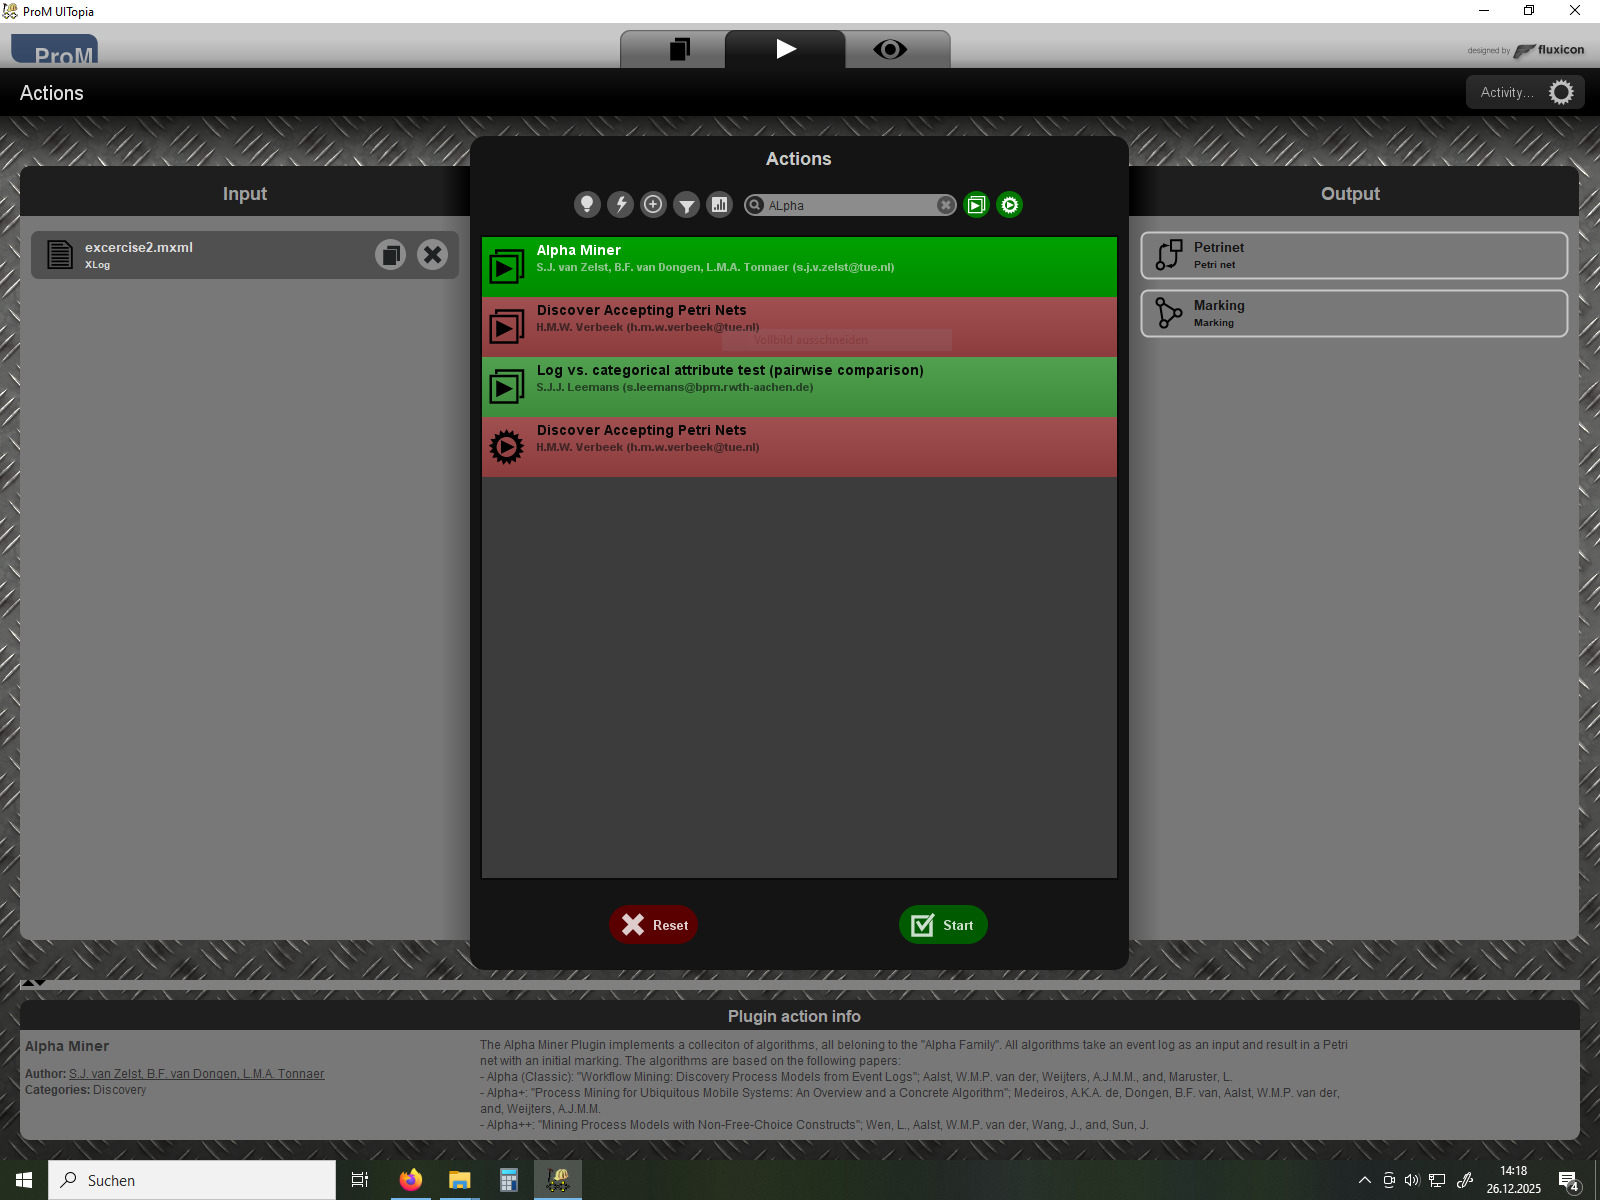
\includegraphics[width=\textwidth]{./figures/related/PromActionInterface.jpeg}
		\caption{ProM actions window showing the selection of the \textit{Alpha Miner} action for an event log, together with the corresponding input and output resources.}
		\label{fig:prom-actions-window}
	\end{subfigure}
	\hfill
	\begin{subfigure}[t]{0.49\textwidth}
		\centering
		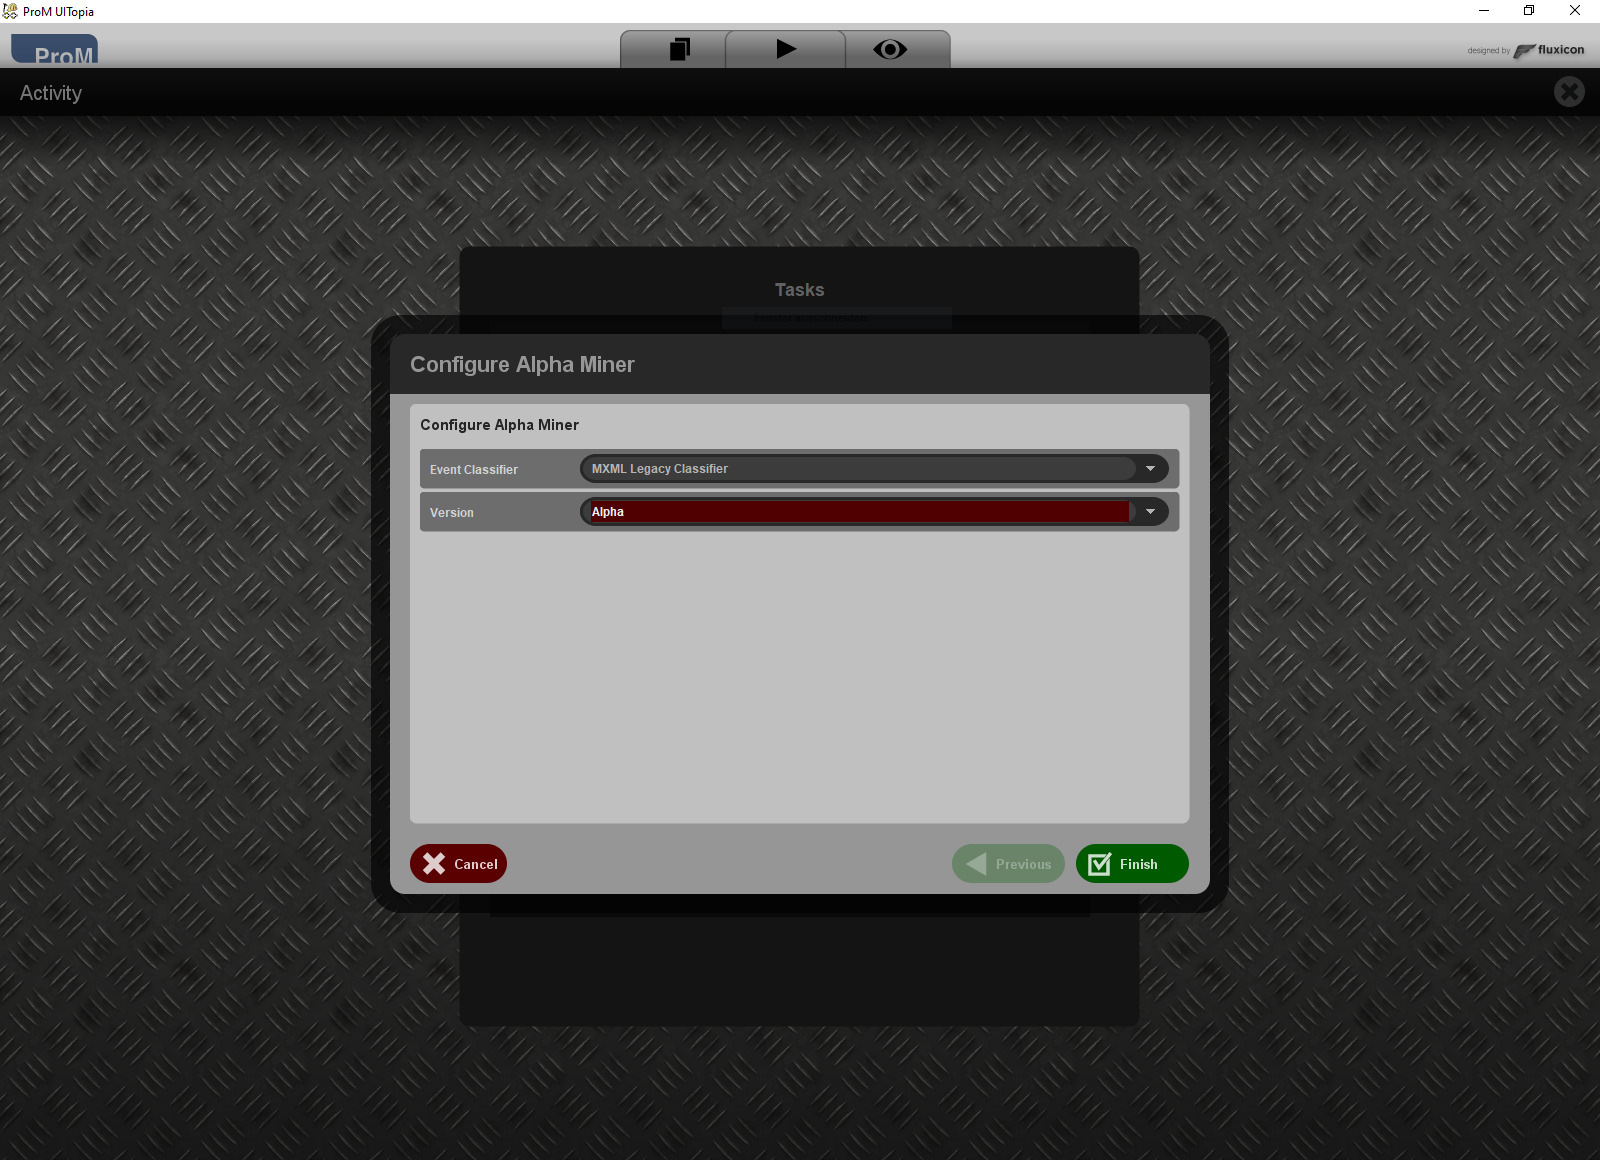
\includegraphics[width=\textwidth]{./figures/related/PromActionUi.jpeg}
		\caption{ProM configuration dialog for the \textit{Alpha Miner} action, showing the available parameter settings before running the action.}
		\label{fig:prom-alpha-miner-config}
	\end{subfigure}
	\caption{ProM user interface for selecting and configuring actions.}
	\label{fig:prom-action-selection-and-config}
\end{figure}

\begin{itemize}
	\item \textbf{Installation difficulties and system dependencies:}
	      ProM depends on Java~8, an older runtime environment that can cause compatibility issues on modern operating systems.
	      Installers are only provided for Windows. The installation process downloads several packages on first launch and often requires restarting the application after installing plugins. ProM also includes many plugins by default, which makes the interface crowded and harder to navigate.

	\item \textbf{Missing documentation and scattered project pages:}
	      The documentation of ProM is limited and partially outdated. Several pages on the official website are empty or no longer maintained. Links to package information and developer guides are often broken, which makes it difficult to find reliable information.

	\item \textbf{High entry barrier for plugin developers:}
	      There is no complete or up-to-date developer guide, and no API reference is linked on the main website. Many existing plugins are complex and are not suitable examples for newcomers. As a result, new developers face a high barrier when trying to extend ProM.

	\item \textbf{Outdated technologies and user interface issues:}
	      ProM relies on legacy technologies and an older user interface framework. The interface does not adapt well to different window sizes and may break at certain resolutions, which makes the tool harder to use.
	\item \textbf{Fragile package management:}
	      Some packages work only with specific ProM versions, and it is often unclear which combinations are correct. Even recent plugins may fail at runtime.
	      For example, both plugins tested during the tool review produced a null pointer exception, which is documented in the user forum and has not been resolved.\footnote{\url{https://promforum.win.tue.nl/discussion/1274/null-pointer-exception-when-trying-to-use-concept-drift-plugin}}
\end{itemize}

The official ProM distributions include the standard OCEL package~\cite{ocel2} and two OCEL-related plugins~\cite{oclpm, constraintchecking}. All of them still use the outdated OCEL~1.0 specification. Support for OCEL~2.0 is currently available only in the ProM Nightly build.

\section{KNIME}

KNIME is an open-source data analytics platform that provides a visual data pipelining environment~\cite{knime}. Nodes in KNIME represent individual data processing functions, and they are connected through edges to form larger workflows. Each node specifies its inputs and outputs as tabular data, and edges connect the output tables of one or more nodes to the input tables of others. Nodes may also define a NodeView for visualizing intermediate results and a NodeDialog for configuring parameters.

\begin{figure}[ht]
	\centering
	\begin{subfigure}[t]{0.5\textwidth}
		\centering
		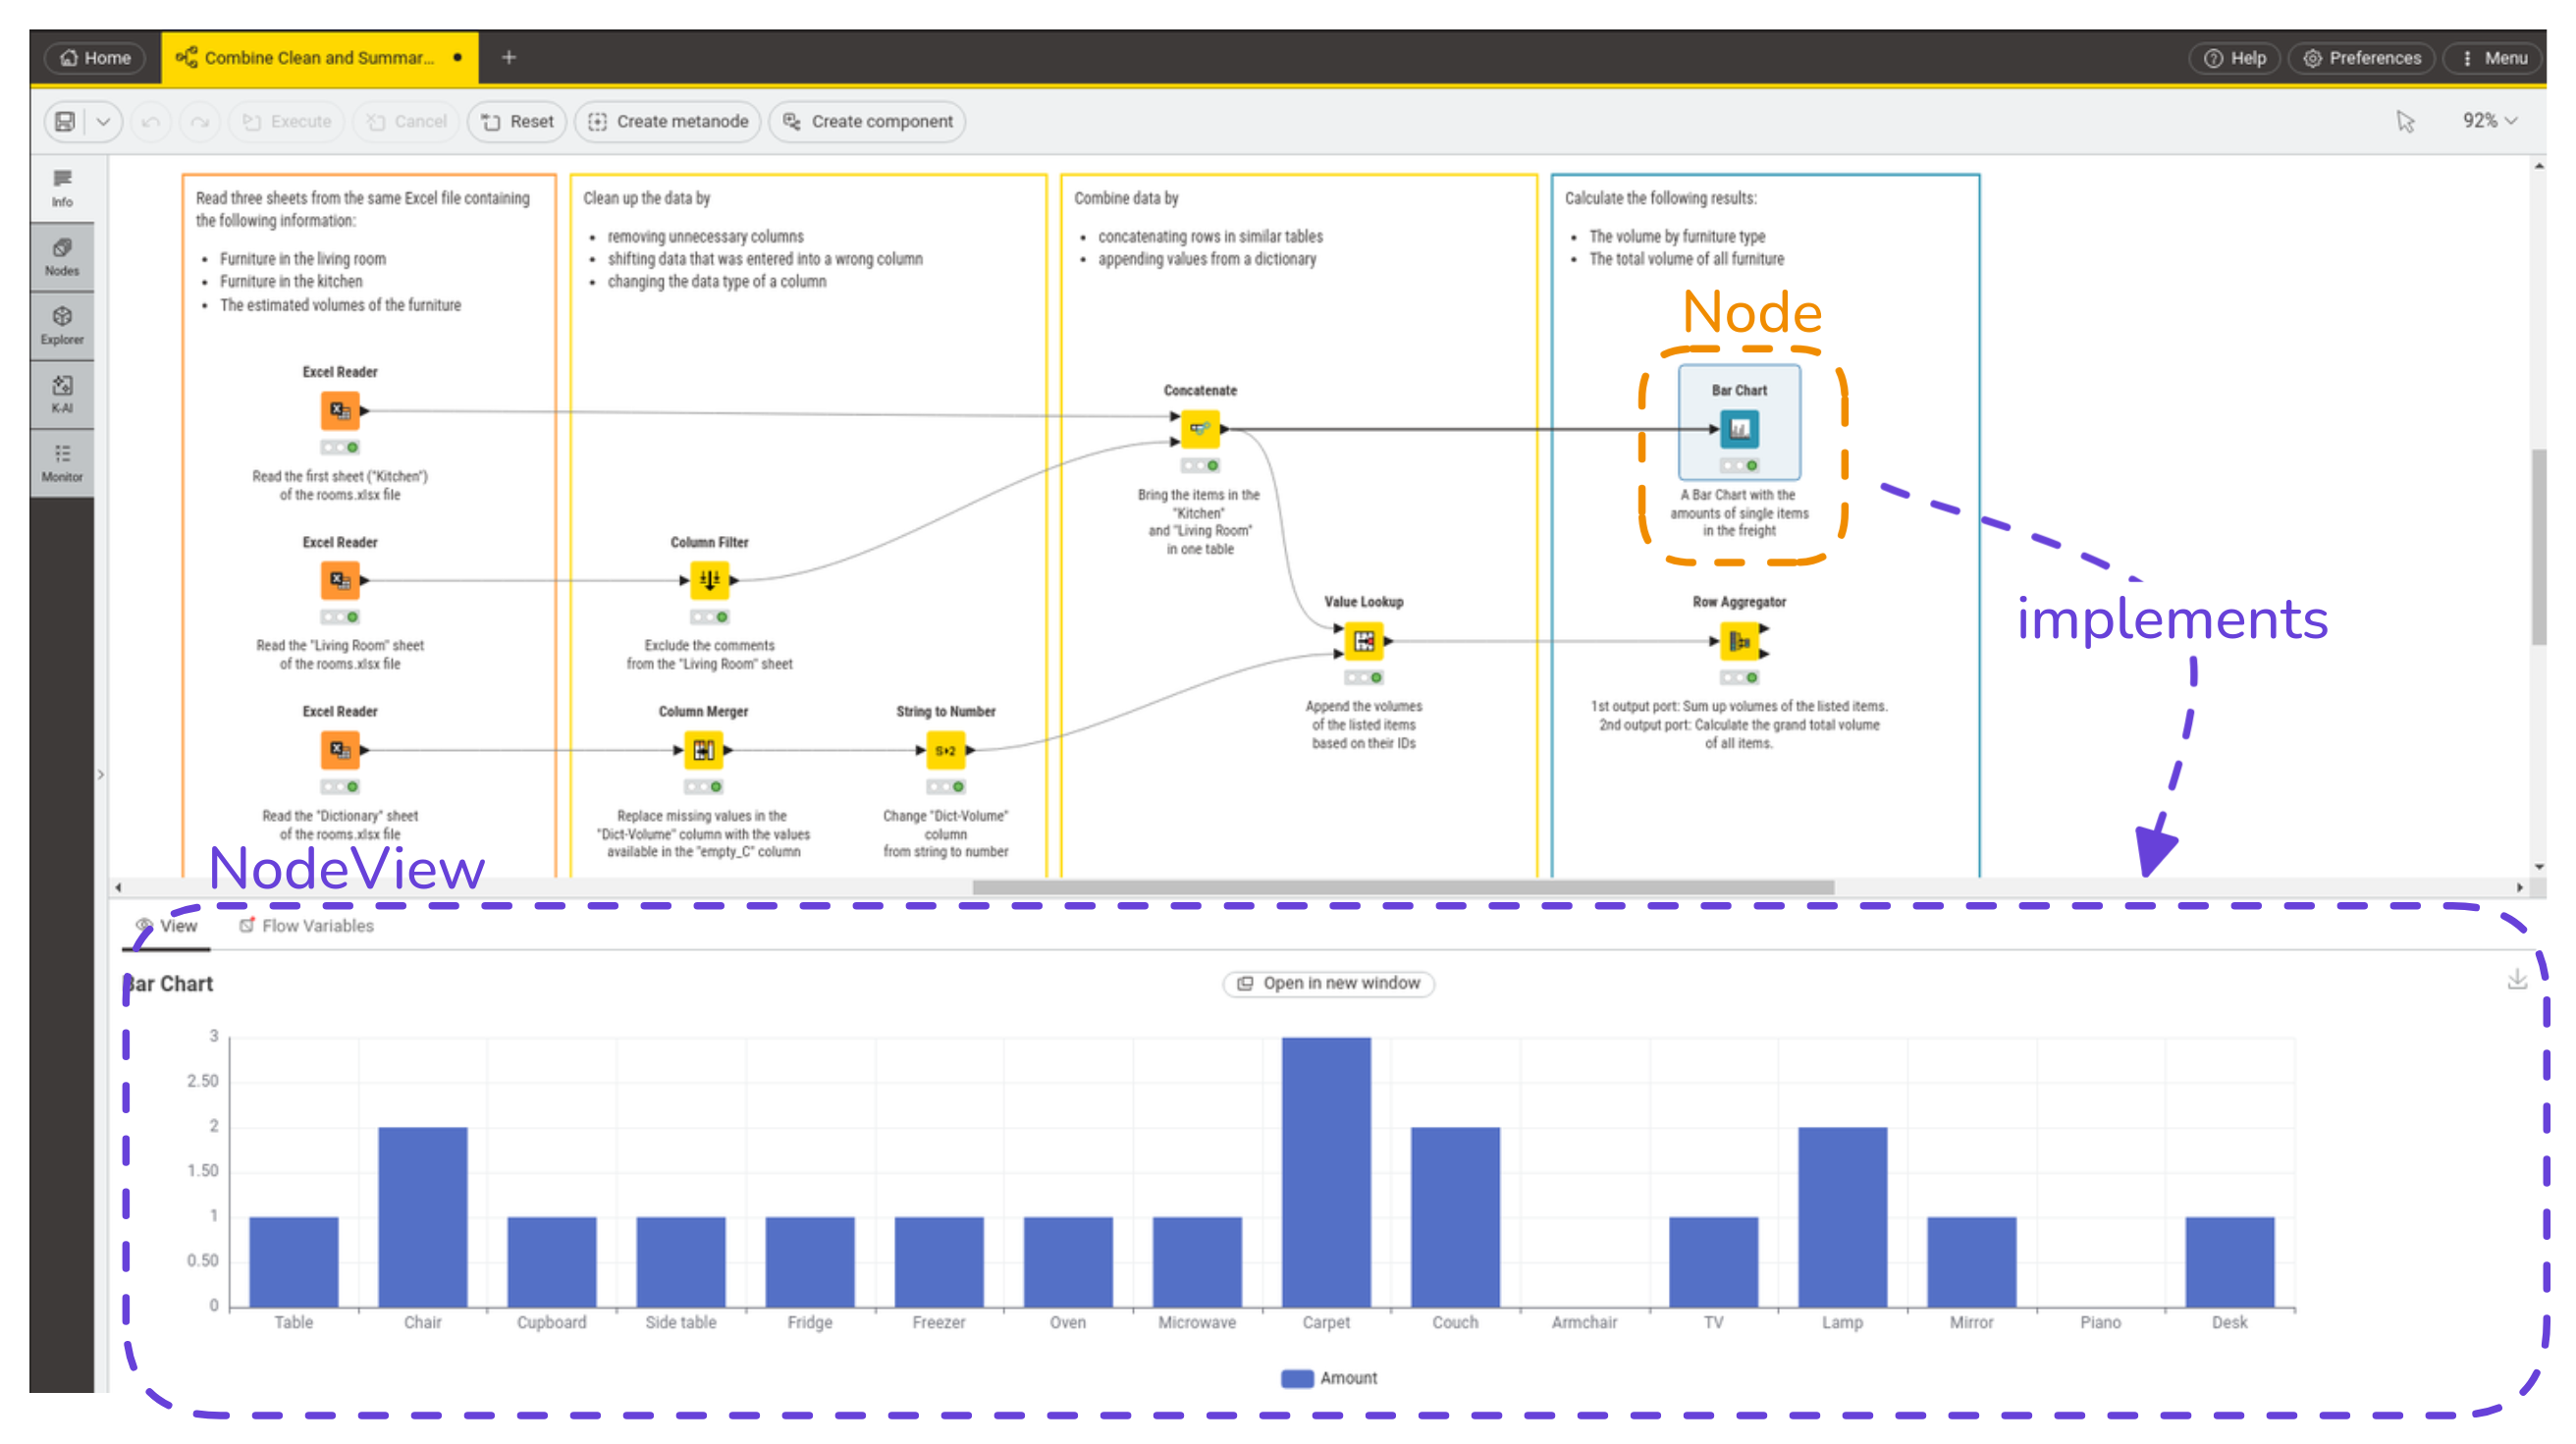
\includegraphics[width=\textwidth]{./figures/related/Knime Nodes.png}
		\caption{KNIME workflow view with connected nodes and an example NodeView for visualizing intermediate results.}
		\label{fig:knime-nodes}
	\end{subfigure}
	\hfill
	\begin{subfigure}[t]{0.31\textwidth}
		\centering
		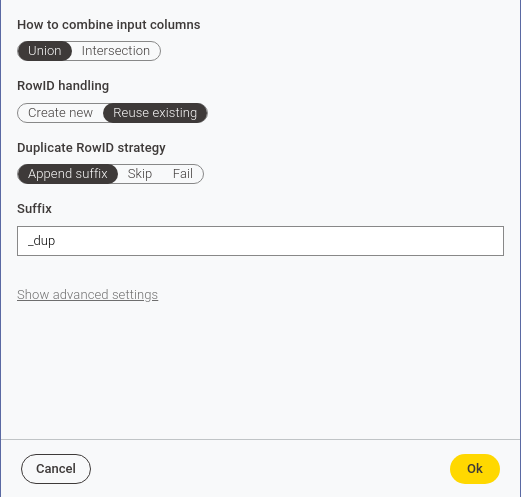
\includegraphics[width=\textwidth]{./figures/related/KNIME_NodeDialog.png}
		\caption{Example NodeDialog used to configure node parameters.}
		\label{fig:knime-node-dialog}
	\end{subfigure}
	\caption{KNIME user interface elements for workflow construction, visualization, and configuration.}
	\label{fig:knime-ui}
\end{figure}

Extensibility is a central principle of the KNIME architecture. The platform can be extended through custom nodes written in Java, and extensions can be shared through the KNIME Community Hub. KNIME also supports integrations with Python and R, which allows external scripts to be embedded into workflows.

Compared to ProM, KNIME offers more extensive and better structured documentation and can be installed through dedicated installers without additional dependencies on all major operating systems. It provides clear guidelines for both users and developers who want to create their own extensions. This makes the development experience more accessible than in ProM, where finding up-to-date documentation is often difficult. Despite its strengths, KNIME imposes constraints through its workflow model. All computations must be expressed as nodes in a workflow, which requires familiarity with KNIME’s concepts and execution model.

Process mining in KNIME is supported through the Process Mining Extension \textit{pm4knime}~\cite{PM4KNIME}. This extension provides nodes for discovery, conformance checking, and filtering, but all functionality is limited to the traditional case-centric setting. It does not include support for object-centric event logs or object-centric algorithms. This lack of OCPM functionality likely explains why object-centric process mining is currently not performed using KNIME.

\section{Celonis Studio}

Celonis Studio is a low-code development environment for building process mining applications. It is designed to support users with limited technical backgrounds, referred to as citizen developers~\cite{celonis}, in creating and using process mining content. Celonis allows data to be ingested from various data sources and transformed into data models that serve as the basis for analysis. From these data models, users can create views that act as dashboards composed of different components. Examples include charts, tables, filters, KPI cards, process visualizations, and input elements such as buttons. These components can be arranged and nested within layout elements to form complete dashboards. Views can then be published as applications in the Celonis Marketplace.

\begin{figure}[ht]
	\centering
	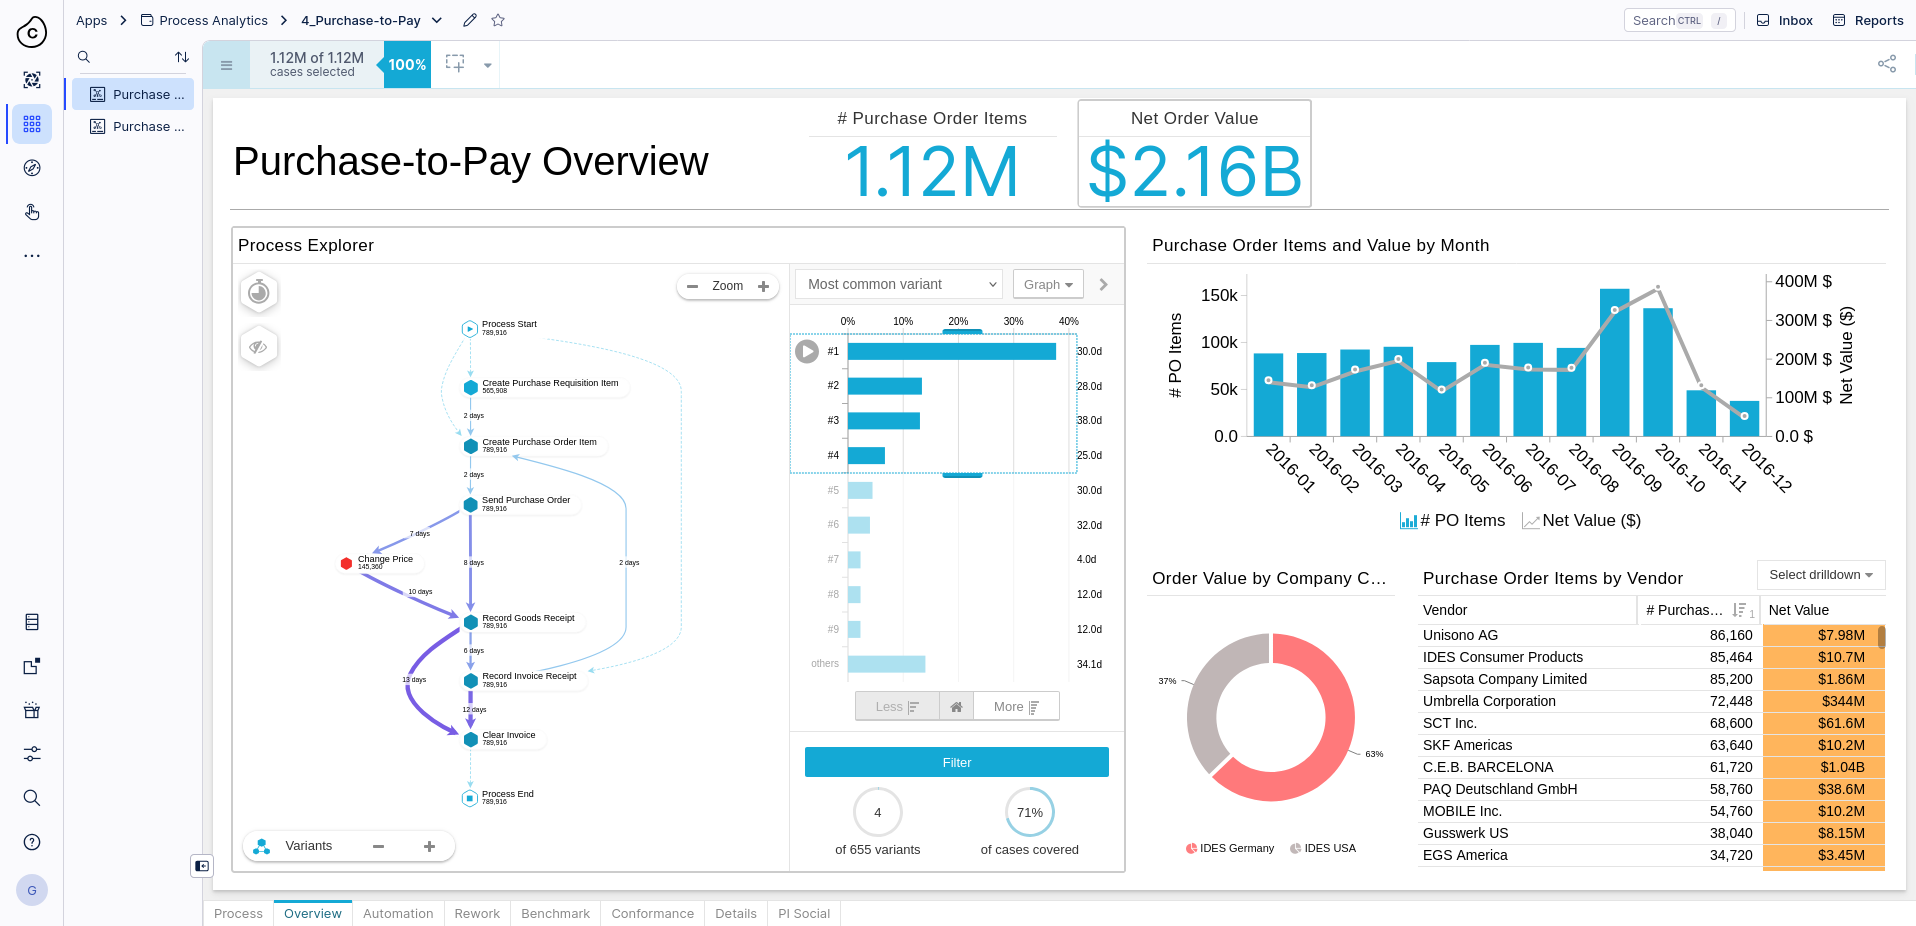
\includegraphics[width=\textwidth]{./figures/related/Celonis.png}
	\caption{Example Celonis Studio dashboard view, combining a process visualization with KPI cards, charts, tables, and filter components.}
	\label{fig:celonis-studio-dashboard}
\end{figure}

Celonis also provides object-centric process mining functionality and includes features that are not available in many other process mining tools.

The documentation for Celonis Studio is extensive, although the overall complexity of the platform requires some effort to get started.
While Celonis offers a powerful querying language for defining metrics and KPIs, users are restricted to the set of view components that the platform provides.
This limits the ability to implement new object-centric process mining techniques directly inside Studio.
Celonis allows Python execution through dedicated components, but this is primarily intended for machine learning tasks on the integrated data rather than for customizing process mining logic.

As a commercial platform, Celonis is not accessible to all users. Access requires a commercial license.

In summary, Celonis is best suited for users who are familiar with the platform and can build interactive dashboards that stay synchronized with the underlying data. End users can access these dashboards through the web without needing technical knowledge.
